\subsection{Sensoren}
\subsubsection{Klassendiagram}
Het doel van de klassen die de sensoren uitlezen is om een structuur op te zetten waarbij zo gemakkelijk mogelijk nieuwe sensoren vervangen/toegevoegd kunnen worden. Ook is het van belang dat van buiten af voor het meten van alle sensoren maar één functie aangeroepen hoeft worden. Hierom is er voor gekozen om de zogeheten CSensorManager aan te maken. Dit is een singleton omdat er altijd maar één manager aangemaakt mag worden in het programma. Aan deze manager kunnen een x aantal sensoren toegevoegd worden.
\vspace{1em}
Wanneer de \emph{mMeasure()} member aangeroepen wordt zal iedere sensor uitgemeten worden. Het resultaat van iedere sensor is beschreven in een SensorOutput map. Deze worden gecombineerd in het Measurements datatype, dit wordt door de \emph{mMeasure()} functie.
\vspace{1em}
Om ieder type sensor te ondersteunen is er een \emph{CSensor} klasse aangemaakt die de minimale functionaliteit van iedere sensor beschrijft, een daadwerkelijke sensor klasse erft deze klasse en kan toegevoegd aan de sensor manager. De \emph{m\_InitCallback()} en \emph{m\_MeasureCallback()} members zijn virtual en worden gebruikt om de sensor specifieke functies van een sensor te implementeren. Iedere \emph{CSensor} heeft ook een \emph{m\_Status} property van het type \emph{CSensorStatus} waarin de status van de sensor opgeslagen is.

\begin{figure}[H]
  \centering
  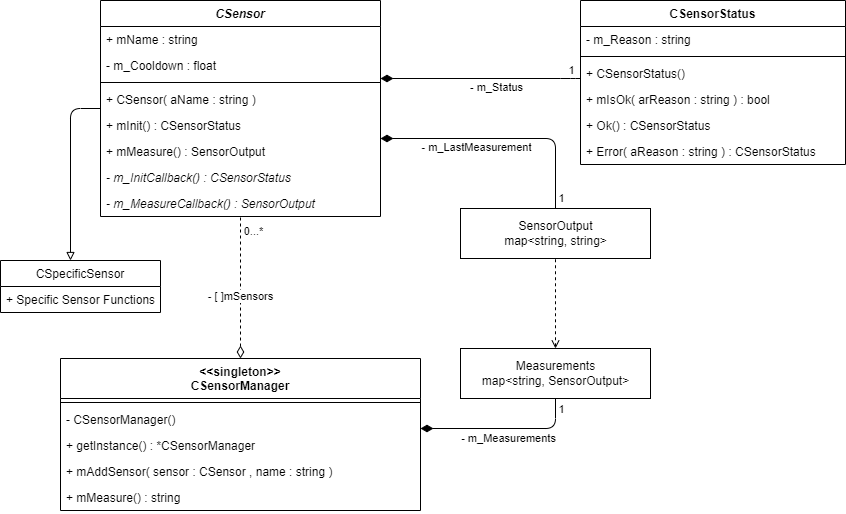
\includegraphics[width=\columnwidth]{uml/sensor-abstraction.png}
\end{figure}

\newpage
\subsubsection{Toestandsdiagram}
De klassen hebben een aantal states waarin de klasse kan verblijven. Over de grootste tijd zullen ze in de idle state staan omdat we slechts één keer per minuut meten. Het meten kan alleen gedaan worden als er al een sensor toegevoegd is aan de sensor manager. Het initialiseren van een sensor gebeurt buiten de sensor manager, een sensor mag alleen toegevoegd worden als de status van de status geen error is.
\vspace{1em}
Het meten van een sensor mag één keer fout gaan, hierdoor wordt er ook een warning in de log opgeschreven. Als hierna het meten van de sensor weer niet goed gaat zal er een error opgeslagen worden in de sensor klasse. Deze status zal later uitgelezen en gelogd moeten worden voordat de metingen opgestuurd worden naar het IoT platform.
\vspace{1em}
Het opslaan van de gemeten waarden kan op twee manieren. Bij voorkeur gaat dit via een bericht met alle getemeten waarden over het internet zodat de waarden direct in het IoT platform staan. Mocht de SenseBox geen actieve internet verbinding hebben wordt de data alsnog in een log bestand op de interne SD kaart opgeslagen zodat deze informatie later alsnog uitgelezen kan worden.

\begin{figure}[H]
  \centering
  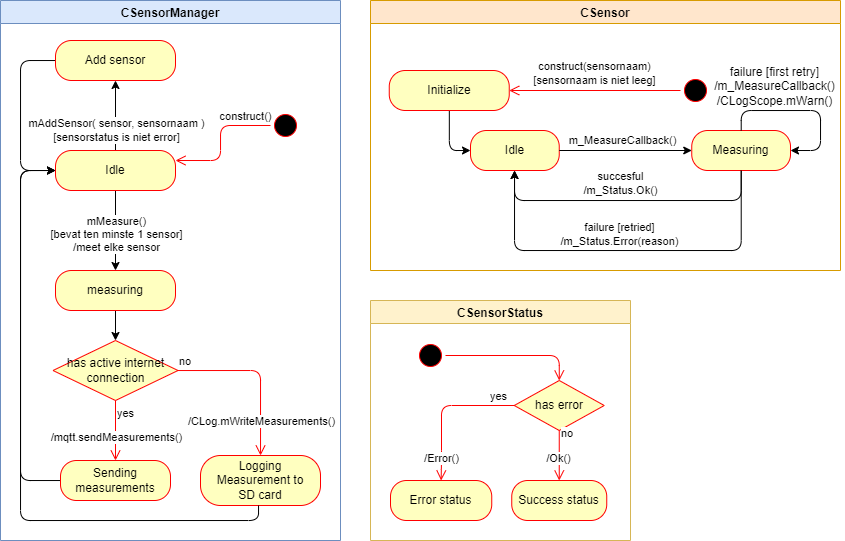
\includegraphics[width=\columnwidth]{uml/sensor-state-diagram.png}
\end{figure}